\subsection*{Problema 04}

\textbf{Enunciado:} Calcular la integral:
\begin{align*}
    I = \int \dfrac{dx}{1 + \cos x}
\end{align*}

\textbf{Solución:} Para resolver esta integral, utilizamos la identidad trigonométrica del ángulo medio sugerida, la cual establece que:
\begin{align*}
    1 + \cos x = 2\cos^2\left(\dfrac{x}{2}\right)
\end{align*}

Sustituyendo esta identidad en el denominador de la integral original, obtenemos:
\begin{align*}
    I &= \int \dfrac{dx}{2\cos^2\left(\frac{x}{2}\right)} \\
    I &= \dfrac{1}{2} \int \dfrac{dx}{\cos^2\left(\frac{x}{2}\right)}
\end{align*}

Recordando que la secante es el recíproco del coseno, es decir, $\sec(\theta) = \frac{1}{\cos(\theta)}$, reescribimos la expresión en términos de la función secante al cuadrado:
\begin{align*}
    I = \dfrac{1}{2} \int \sec^2\left(\dfrac{x}{2}\right) dx
\end{align*}

Para resolver esta nueva integral, aplicamos el método de sustitución simple. Definimos la variable $u$ y su diferencial:
\begin{align*}
    u &= \dfrac{x}{2} \\
    du &= \dfrac{1}{2} dx \implies dx = 2 du
\end{align*}

Sustituyendo $u$ y $dx$ en la integral, tenemos:
\begin{align*}
    I &= \dfrac{1}{2} \int \sec^2(u) (2 du) \\
    I &= \int \sec^2(u) du
\end{align*}

La antiderivada estándar de la función secante cuadrada es la función tangente. Por lo tanto, integramos directamente:
\begin{align*}
    I = \tan(u) + C
\end{align*}

Finalmente, regresamos a la variable original $x$ sustituyendo $u = \frac{x}{2}$ y agregamos la constante de integración $C$:
\begin{align*}
    I = \tan\left(\dfrac{x}{2}\right) + C
\end{align*}

\begin{figure}[H]
	\centering
	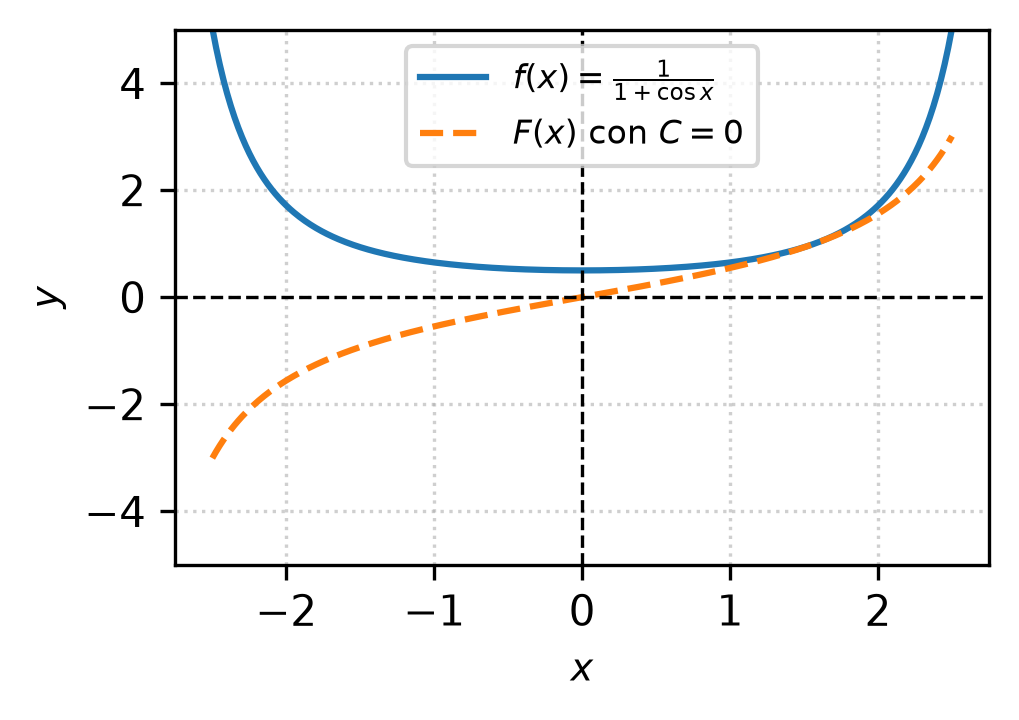
\includegraphics[width=\columnwidth]{semana_04/graficas/SEM04_P04_grafica.png}
	\caption{Representación gráfica de $f(x)$ y su antiderivada $F(x)$ evaluada para la constante de integración $C = 0$ (Problema 04).}
	\label{fig:problema04}
\end{figure}
